\section{System Integration}
\label{sec:system_integration}

This chapter describes the detailed integration plan for the Best Bike Paths system, categorized by the integration levels defined in \Cref{sec:integration_strategy}.

\subsection{Data Layer Integration}
Integration of the DBMS and Cache components ensures data persistence and consistency.
\begin{itemize}
    \item \textbf{DBMS Integration:} Validates schema correctness, constraints (PK/FK), and transaction management in PostgreSQL.
    \item \textbf{Cache Integration:} Verifies Redis connection, cache hit/miss logic, and invalidation strategies upon data updates.
\end{itemize}

\subsection{Service Layer Integration}
Integration of backend microservices with the data layer and each other.
\begin{itemize}
    \item \textbf{User Management:} Integrates with User Repository and Email Service. Validates registration, login, and profile updates.
    \item \textbf{Trip Management:} Integrates with Trip Repository and Sensor Data Service. Handling of manual and automated trip recording.
    \item \textbf{Path Management:} Integrates with PostGIS for spatial queries. Manages path lifecycle (Draft $\to$ Published).
    \item \textbf{Sensor Data Processing:} Consumes data from RabbitMQ, processes GPS streams, and persists path segments.
    \item \textbf{Rating Service:} Links ratings to Paths and Users, ensuring referential integrity.
\end{itemize}

\subsection{API Gateway Integration}
The API Gateway acts as the single entry point. Integration focus:
\begin{itemize}
    \item \textbf{Routing:} Requests (\texttt{/users}, \texttt{/paths}) are forwarded to the correct service.
    \item \textbf{Auth Middleware:} Validates JWT tokens and enforces authorization policies.
    \item \textbf{Error Handling:} Standardizes error responses (4xx, 5xx) for the client.
\end{itemize}

\subsection{External Services Integration}
Integration with third-party APIs using mocks for reliability.
\begin{itemize}
    \item \textbf{Weather API:} Fetches weather conditions for trips. Mocks simulate valid data and timeouts.
    \item \textbf{Map Service:} Provides geocoding and tiles. Mocks ensure consistent responses without external costs.
    \item \textbf{Email Service:} Simulates email sending (verification, reset) without actual delivery in test environments.
\end{itemize}

\subsection{Client Integration}
Integration of the mobile app with the backend.
\begin{itemize}
    \item \textbf{Mobile Core:} Validates UI rendering, navigation, and API client communication.
    \item \textbf{Sensor Manager:} Manages device sensors (GPS, Gyroscope) and feeds data to the app logic.
    \item \textbf{Trip Detection:} Algorithms process sensor streams to detect starts/stops and upload trip data.
\end{itemize}

\subsection{End-to-End Integration}
Validates complete user flows from Client to DB.
\begin{itemize}
    \item \textbf{Critical Use Cases:} User Registration (UC1), Login (UC2), Manual Path Insertion (UC3), Path Search (UC6).
    \item \textbf{Advanced Use Cases:} Automated Path Insertion (UC4), Path Publishing (UC5), Reviews (UC7), Personal Trips (UC8).
\end{itemize}

\subsection{Integration Sequence Diagrams}
\label{subsec:integration_sequence_diagrams}

The following sequence diagrams illustrate key integration flows.

\subsubsection{Service-to-Database Integration}
A generic write flow (e.g., creating a user or path) involves the Service calling the Repository, which persists to PostgreSQL and invalidates the Redis cache.

\begin{figure}[ht]
    \centering
    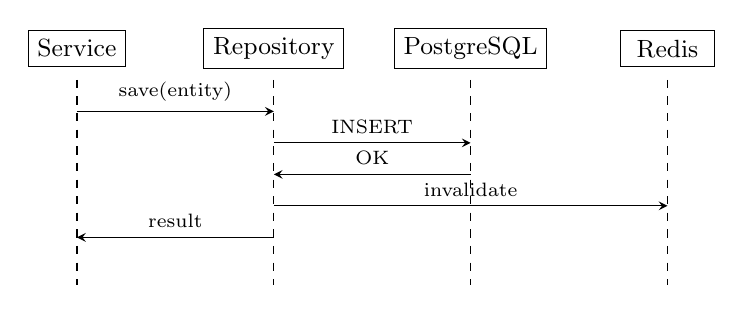
\begin{tikzpicture}[
        every node/.style={font=\small},
        participant/.style={rectangle, draw, minimum width=1.2cm, minimum height=0.45cm},
        arrow/.style={->, >=stealth}
    ]
        \node[participant] (service) at (0,0) {Service};
        \node[participant] (repo) at (2.5,0) {Repository};
        \node[participant] (db) at (5.0,0) {PostgreSQL};
        \node[participant] (cache) at (7.5,0) {Redis};

        \draw[dashed] (0, -0.4) -- (0, -3.0);
        \draw[dashed] (2.5, -0.4) -- (2.5, -3.0);
        \draw[dashed] (5.0, -0.4) -- (5.0, -3.0);
        \draw[dashed] (7.5, -0.4) -- (7.5, -3.0);

        \draw[arrow] (0, -0.8) -- (2.5, -0.8) node[midway, above, font=\scriptsize] {save(entity)};
        \draw[arrow] (2.5, -1.2) -- (5.0, -1.2) node[midway, above, font=\scriptsize] {INSERT};
        \draw[arrow] (5.0, -1.6) -- (2.5, -1.6) node[midway, above, font=\scriptsize] {OK};
        \draw[arrow] (2.5, -2.0) -- (7.5, -2.0) node[midway, above, font=\scriptsize] {invalidate};
        \draw[arrow] (2.5, -2.4) -- (0, -2.4) node[midway, above, font=\scriptsize] {result};
    \end{tikzpicture}
    \caption{Service-to-Database Integration Flow}
    \label{fig:seq_service_db}
\end{figure}

\subsubsection{Service-to-Service Integration}
Example: Path Search Service calls Path Management Service to resolve path details for search results.

\begin{figure}[ht]
    \centering
    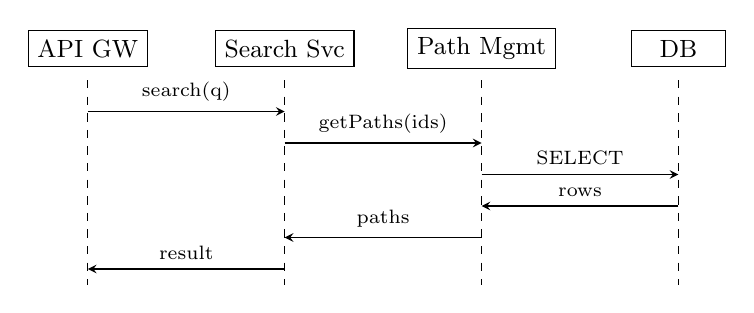
\begin{tikzpicture}[
        every node/.style={font=\small},
        participant/.style={rectangle, draw, minimum width=1.2cm, minimum height=0.45cm},
        arrow/.style={->, >=stealth}
    ]
        \node[participant] (gw) at (0,0) {API GW};
        \node[participant] (search) at (2.5,0) {Search Svc};
        \node[participant] (mgmt) at (5.0,0) {Path Mgmt};
        \node[participant] (db) at (7.5,0) {DB};

        \draw[dashed] (0, -0.4) -- (0, -3.0);
        \draw[dashed] (2.5, -0.4) -- (2.5, -3.0);
        \draw[dashed] (5.0, -0.4) -- (5.0, -3.0);
        \draw[dashed] (7.5, -0.4) -- (7.5, -3.0);

        \draw[arrow] (0, -0.8) -- (2.5, -0.8) node[midway, above, font=\scriptsize] {search(q)};
        \draw[arrow] (2.5, -1.2) -- (5.0, -1.2) node[midway, above, font=\scriptsize] {getPaths(ids)};
        \draw[arrow] (5.0, -1.6) -- (7.5, -1.6) node[midway, above, font=\scriptsize] {SELECT};
        \draw[arrow] (7.5, -2.0) -- (5.0, -2.0) node[midway, above, font=\scriptsize] {rows};
        \draw[arrow] (5.0, -2.4) -- (2.5, -2.4) node[midway, above, font=\scriptsize] {paths};
        \draw[arrow] (2.5, -2.8) -- (0, -2.8) node[midway, above, font=\scriptsize] {result};
    \end{tikzpicture}
    \caption{Service-to-Service Integration Flow}
    \label{fig:seq_service_service}
\end{figure}

\subsubsection{Client-Server Integration}
Authenticated Request Flow: Login $\to$ Token Storage $\to$ API Request.

\begin{figure}[ht]
    \centering
    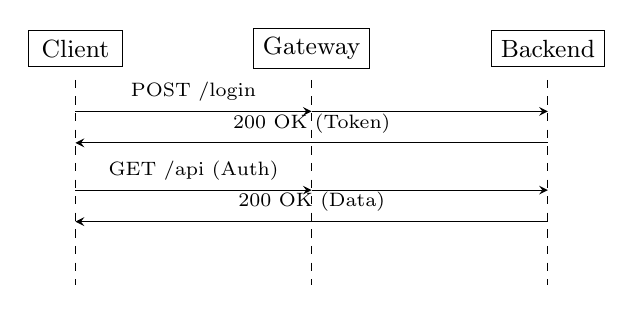
\begin{tikzpicture}[
        every node/.style={font=\small},
        participant/.style={rectangle, draw, minimum width=1.2cm, minimum height=0.45cm},
        arrow/.style={->, >=stealth}
    ]
        \node[participant] (client) at (0,0) {Client};
        \node[participant] (gw) at (3.0,0) {Gateway};
        \node[participant] (backend) at (6.0,0) {Backend};

        \draw[dashed] (0, -0.4) -- (0, -3.0);
        \draw[dashed] (3.0, -0.4) -- (3.0, -3.0);
        \draw[dashed] (6.0, -0.4) -- (6.0, -3.0);

        \draw[arrow] (0, -0.8) -- (3.0, -0.8) node[midway, above, font=\scriptsize] {POST /login};
        \draw[arrow] (3.0, -0.8) -- (6.0, -0.8);
        \draw[arrow] (6.0, -1.2) -- (0, -1.2) node[midway, above, font=\scriptsize] {200 OK (Token)};
        \draw[arrow] (0, -1.8) -- (3.0, -1.8) node[midway, above, font=\scriptsize] {GET /api (Auth)};
        \draw[arrow] (3.0, -1.8) -- (6.0, -1.8);
        \draw[arrow] (6.0, -2.2) -- (0, -2.2) node[midway, above, font=\scriptsize] {200 OK (Data)};
    \end{tikzpicture}
    \caption{Client-Server Authenticated Flow}
    \label{fig:seq_client_server}
\end{figure}
